\documentclass[11pt]{article}

% Packages
\usepackage{graphicx}   % For including figures
\usepackage{geometry}   % For page margins
\usepackage{hyperref}   % For clickable links and URLs

% Layout settings
\geometry{margin=1in}   % 1-inch margins all around
\linespread{1.1}        % Slightly looser line spacing for readability


\title{\textbf{Predicting Auto Insurance Claim Likelihood Using Ensemble Learning Under Extreme Class Imbalance}}
\author{
Sukaina D. Alkhalidy \\
\texttt{alkhal13@msu.edu} \\
October 2025 \\
\href{https://github.com/sukaina13/cmse492_project}{https://github.com/sukaina13/cmse492\_project}
}
\date{}

\begin{document}
\maketitle

\section*{Abstract}
Predicting whether an auto insurance policyholder will file a claim in the next year is an important problem for both financial planning and fair risk assessment. This project explores how machine learning can improve claim prediction using the Porto Seguro Safe Driver dataset, a large and highly imbalanced dataset where only about 3.6\% of policyholders made a claim. I compare simple baseline models such as predicting the majority class and logistic regression with more advanced ensemble methods like Balanced Random Forest and EasyEnsemble, which are designed to handle class imbalance effectively. Preliminary results show that the EasyEnsemble model performs much better at identifying claim cases, increasing recall from 0.00 to around 0.58 and achieving an area under the ROC curve (AUC) of 0.63. These findings suggest that ensemble-based approaches can improve fairness and accuracy in predicting rare insurance claims. Ultimately, this project aims to build interpretable, data-driven models that help insurance companies make more informed and equitable decisions when assessing driver risk.

\section{Background and Motivation}
Predicting whether a driver will file an insurance claim is one of the most important and challenging tasks in the insurance industry. Each year, companies must decide how to set fair premiums while maintaining profitability and protecting customers from unfair pricing. A model that can accurately estimate the likelihood of a claim allows insurers to manage financial risk, detect potential fraud, and better allocate resources for claims investigation. However, the key challenge lies in the data itself—claim events are extremely rare, occurring in only about 3–4\% of all cases, which makes accurate prediction very difficult.

Traditional statistical methods, such as logistic regression and generalized linear models, have long been used in insurance analytics. While these approaches are simple and interpretable, they tend to struggle with highly imbalanced datasets. In cases like this, they often predict the majority class (“no claim”) nearly all the time, resulting in high overall accuracy but poor recall for the minority class—the actual claim cases that matter most. This imbalance leads to models that appear strong on paper but fail in real-world decision-making, where missing a true claim can have significant financial costs.

Machine learning offers more powerful ways to handle this challenge. Ensemble-based models such as Balanced Random Forest and EasyEnsemble are specifically designed to correct class imbalance by training on balanced subsets of data and aggregating results. These methods can detect rare claim cases more effectively while maintaining generalization. They also provide interpretable outputs, such as feature importance scores, that can help explain which policyholder or vehicle characteristics are most predictive of risk.

The goal of this project is to develop and evaluate such ensemble learning models to improve the accuracy and fairness of claim prediction. By comparing baseline models (like logistic regression and majority class prediction) with advanced ensemble methods, this work aims to demonstrate how data-driven approaches can enhance risk modeling and provide actionable insights for insurance companies.

\section{Data Description}
The dataset used in this project originates from Porto Seguro, one of Brazil’s largest auto and home insurance companies. It was released as part of the 2017 Kaggle competition \textit{“Porto Seguro’s Safe Driver Prediction”}, organized by data scientists Addison Howard, Adriano Moala, and Walter Reade. The competition challenged participants to build models that predict the probability that a policyholder will file an auto insurance claim in the following year. The data was collected internally by Porto Seguro through historical customer records, vehicle information, and claim history, and was shared to encourage innovation in risk modeling. The dataset’s goal was to improve claim prediction accuracy so insurers could offer fairer pricing—lower premiums for safe drivers and more accurate risk assessment for higher-risk individuals.

The training dataset contains 595,212 records and 59 variables, including 58 predictive features and one target variable (\texttt{target}). Features cover several categories:
\begin{itemize}
    \item Demographic and personal data (e.g., \texttt{ps\_ind\_*})
    \item Vehicle attributes (e.g., \texttt{ps\_car\_*})
    \item Geographical and regional risk indicators (e.g., \texttt{ps\_reg\_*})
    \item Calculated or engineered risk scores (e.g., \texttt{ps\_calc\_*})
\end{itemize}

Most variables are numerical, while some are binary or categorical. The target variable is binary, indicating whether a claim was filed (1) or not (0). From an exploratory analysis, the dataset shows a severe class imbalance, with only 3.6\% of the policyholders filing claims. Missing values are concentrated in a few variables, such as \texttt{ps\_car\_03\_cat} (69\% missing) and \texttt{ps\_car\_05\_cat} (45\% missing). The majority of other features are complete and exhibit reasonable distributions without extreme outliers.

Two key figures illustrate the dataset’s structure and challenges:
\begin{itemize}
    \item \textbf{Figure 1:} Percentage of missing values across key features.
    \item \textbf{Figure 2:} Target variable distribution showing extreme class imbalance.
\end{itemize}

Preprocessing steps include imputing missing values using the median for numerical variables and the mode for categorical variables, dropping features with more than 50\% missingness, encoding categorical variables using label encoding, and preserving the natural feature scales since tree-based ensemble models are invariant to normalization. Together, these steps prepare the dataset for robust model training while maintaining interpretability and minimizing bias introduced by imbalanced data.

\section{Proposed Methodology}
This project uses a supervised machine learning approach to predict whether a driver will file an insurance claim within the next year. Since this is a binary classification problem, the main goal is to train models that can accurately identify the small number of claim cases while avoiding bias toward the majority “no claim” class.

To study how model complexity affects performance, three models will be compared:
\begin{enumerate}
    \item \textbf{Majority Class Baseline:} Always predicts the most common outcome (“no claim”). This provides a simple benchmark to show how misleading accuracy can be in imbalanced datasets.
    \item \textbf{Logistic Regression (Weighted):} A linear classifier that’s easy to interpret and fast to train. By applying class weights, it compensates for the imbalance in the data, giving more importance to the minority class.
    \item \textbf{Ensemble Models – Balanced Random Forest and EasyEnsembleClassifier:} Nonlinear methods that train on balanced subsets of the data and aggregate predictions, improving recall and robustness for rare classes.
\end{enumerate}

In terms of complexity:
\begin{itemize}
    \item The baseline has no parameters or learning ability.
    \item Logistic Regression is a low-complexity linear model.
    \item Ensemble models capture deeper feature interactions via multiple trees and boosting layers.
\end{itemize}

The general workflow includes:
\begin{enumerate}
    \item Load and clean the dataset (handle missing values, encode features).
    \item Perform a stratified train/validation/test split to preserve class balance.
    \item Train and tune each model using cross-validation.
    \item Evaluate results using accuracy, precision, recall, F1-score, and ROC-AUC.
    \item Visualize performance with ROC curves, confusion matrices, and feature importance charts.
\end{enumerate}

This structured comparison highlights how more advanced ensemble methods can significantly improve recall and AUC in highly imbalanced classification problems, making the results more useful for real-world insurance risk prediction.

\section{Evaluation Framework}
Because this dataset is extremely imbalanced, accuracy alone isn’t a good measure of success. A model that always predicts “no claim” would score over 96\% accuracy but completely fail to identify the few real claim cases. For that reason, I’ll evaluate my models using metrics that focus more on detecting the minority class.

\textbf{Metrics:}
\begin{itemize}
    \item \textbf{Recall:} Measures how many actual claim cases are correctly identified. This is the top priority, since missing true claims (false negatives) is worse than overpredicting claims.
    \item \textbf{Precision:} Measures how many of the model’s positive predictions are correct.
    \item \textbf{F1-score:} Balances recall and precision for fair comparison.
    \item \textbf{AUC (ROC):} Evaluates class separability across thresholds, useful for imbalanced data.
\end{itemize}

\textbf{Data Splitting Strategy:}  
A stratified 70/15/15 split ensures balanced class representation across training, validation, and testing. The training set is used to fit models, the validation set for tuning, and the test set for final evaluation.

\textbf{Baseline Comparisons:}  
The baseline model predicts “no claim” for every case. It achieves high accuracy but zero recall and F1-score, clearly showing the need for more sophisticated models. Logistic Regression, Balanced Random Forest, and EasyEnsembleClassifier will be compared against this baseline to measure improvement.

\textbf{Success Criteria:}
\begin{itemize}
    \item Recall $\geq$ 0.55
    \item AUC $\geq$ 0.65
    \item Significant increase in F1-score compared to baseline
\end{itemize}

If these goals are achieved, it will demonstrate that ensemble-based approaches meaningfully improve claim prediction and have practical value for real-world insurance applications.

\section{Timeline and Milestones}
This project will span from late October to December 8, 2025, and is structured into weekly milestones to ensure steady progress. The first week focuses on completing data cleaning, handling missing values, and finalizing exploratory data analysis, including visualizations that highlight feature patterns and data quality.

In early November, I will build and test the baseline models—specifically, the majority-class predictor and logistic regression—before advancing to ensemble methods such as Balanced Random Forest and EasyEnsembleClassifier. By late November, I’ll evaluate performance using recall, F1-score, and AUC while tuning hyperparameters. The final weeks are dedicated to writing the report, preparing the presentation, and reviewing deliverables. Buffer time during Weeks 13–14 is included to manage unexpected challenges such as retraining or runtime issues. The critical path involves model development and evaluation, as these directly impact the final deliverables.

\begin{figure}[h]
    \centering
    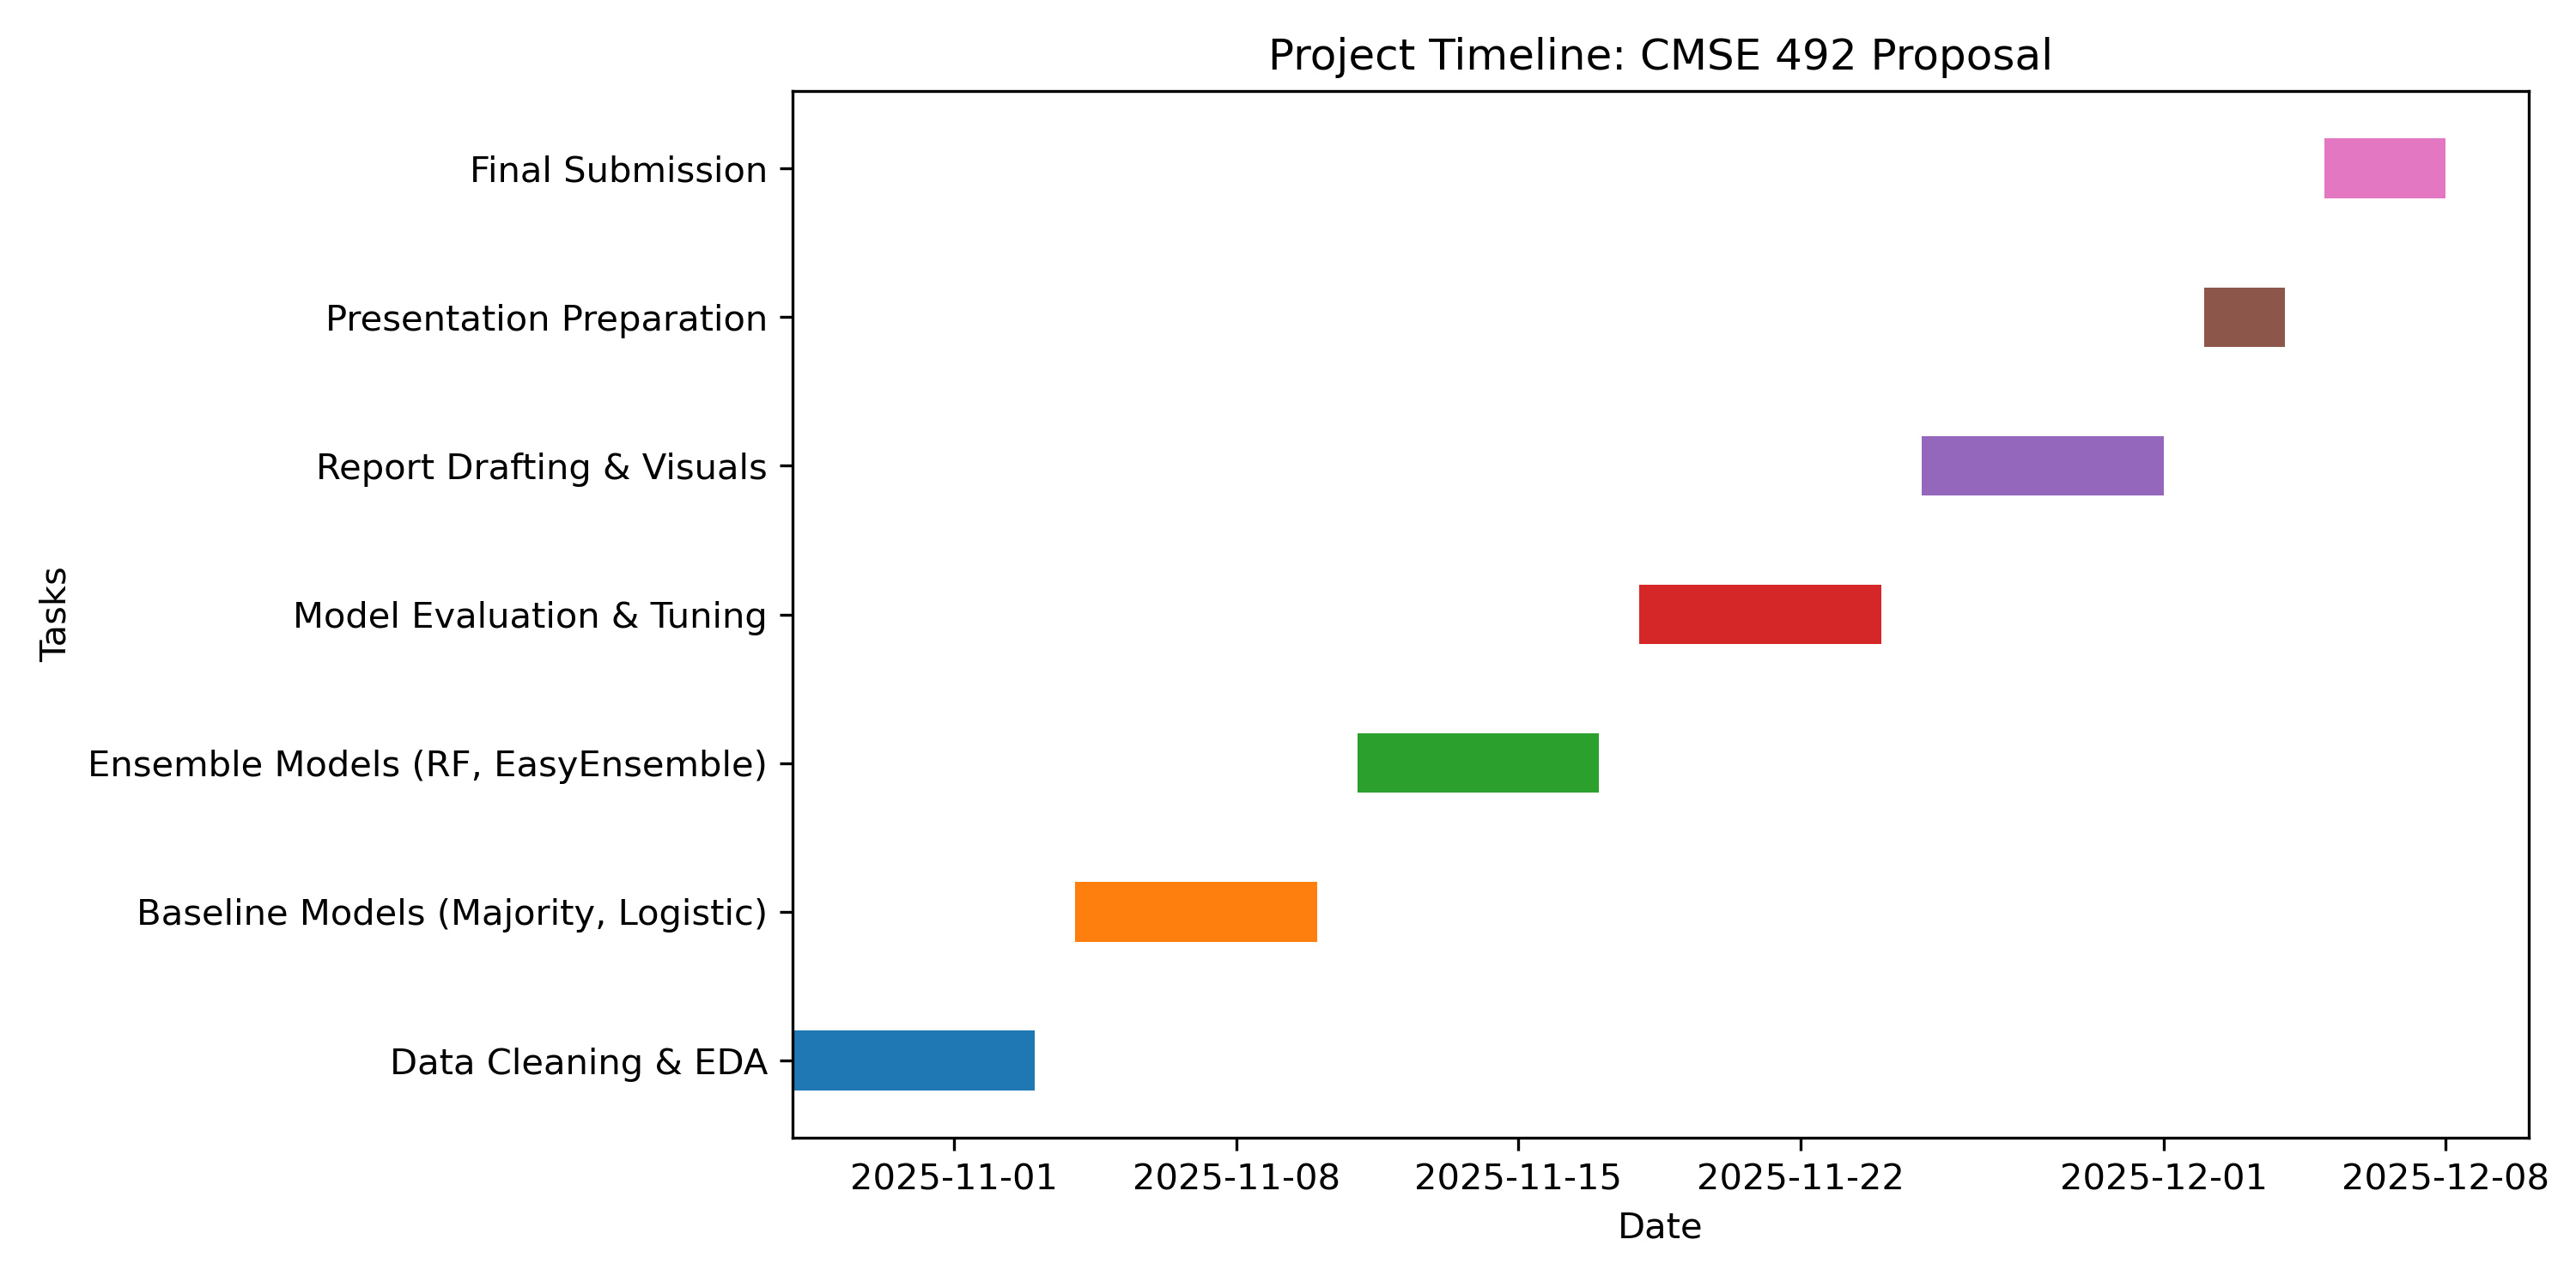
\includegraphics[width=0.9\textwidth]{../figures/gantt_chart.png}
    \caption{Project timeline and milestones for CMSE 492 proposal.}
\end{figure}

\end{document}
